\subsection{Lucas Prati}

\subsubsection{Importazione delle risorse di gioco}
\textbf{Problema}\newline
All'avvio, il gioco deve importare quattro risorse distinte 
(carte JSON, impostazioni YAML, testo delle regole e mazzo di “imprevisti”), ognuna con un formato e un parsing dedicati. 
Se uno di questi file è assente, malformato o non conforme alle specifiche, il caricamento può interrompersi, 
privando l'applicazione dei dati necessari per avviare la partita o provocando comportamenti incoerenti.
\dots\newline
\textbf{Soluzione}\newline
Abbiamo introdotto un'unica astrazione di lettura, \texttt{UseFile}, e poi tre strategie specializzate:\newline
\begin{itemize}
  \item \texttt{UseFileTxt} per il testo semplice,
  \item \texttt{UseFileJson} per gli array JSON,
  \item \texttt{UseConfigurationFile} per le coppie chiave-valore del file di configurazione.
\end{itemize}
Ciascuna strategia viene implementata in una classe dedicata — \texttt{UseFileTxtImpl, UseFileJsonImpl, UseConfigurationFileImpl} — 
che utilizza un helper comune (\texttt{AbstractUseFileImpl}) il quale centralizza apertura e chiusura delle risorse, 
lasciando alle classi implementative solo il compito di trasformare i dati grezzi nel formato richiesto.\newline
In questo modo il resto dell'applicazione rimane completamente agnostico sull'estrazione dei dati da file: 
seleziona la strategia corretta e invoca il metodo di caricamento senza occuparsi dei dettagli di I/O o di parsing.\newline
\begin{figure}[H]
    \centering
    \makebox[1.0\textwidth]{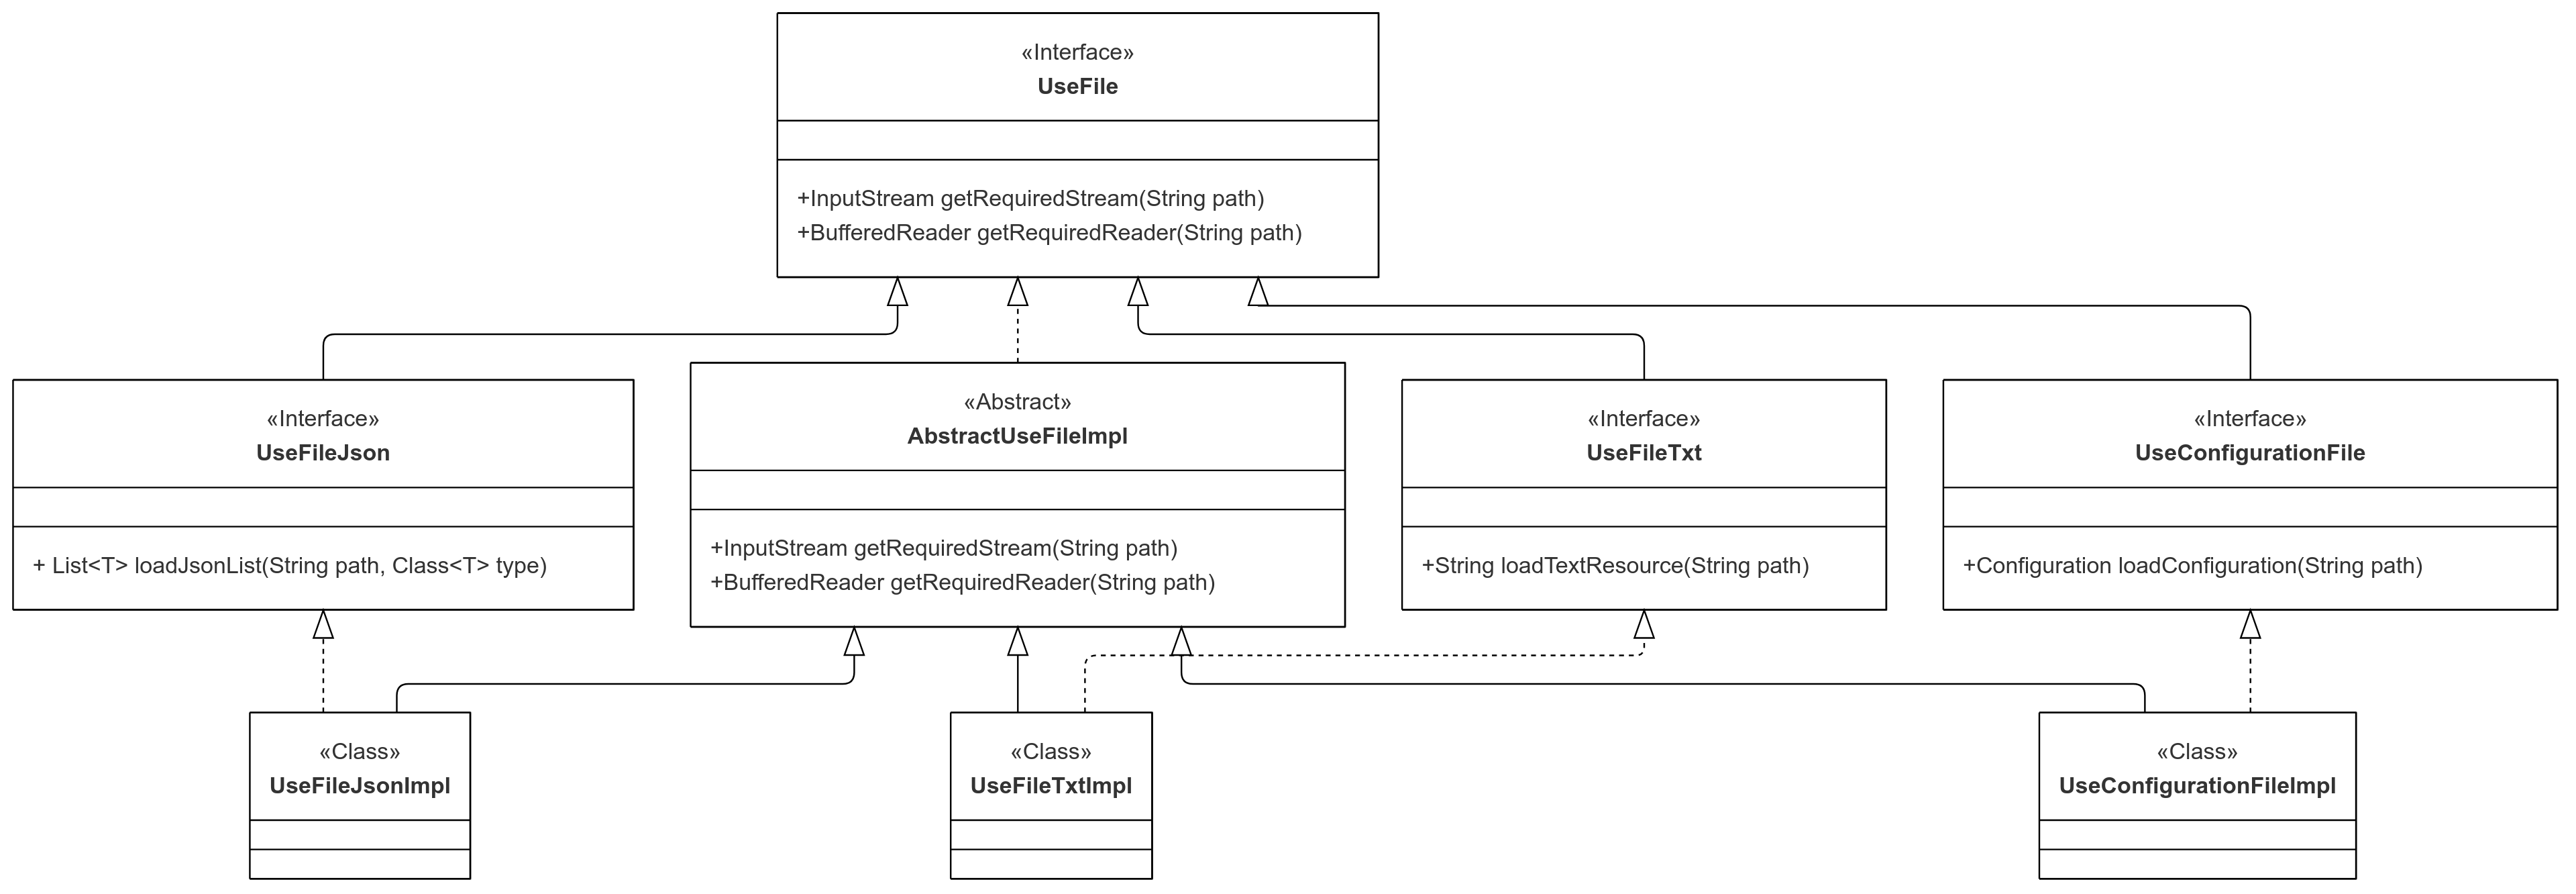
\includegraphics[width=1.3\textwidth]{img/prati/UseFile.png}}	
    \caption{Schema UML dell'importazione delle risorse di gioco}
	\label{img:UseFile}
\end{figure}

\subsubsection{Creazione delle tessere di gioco}
\textbf{Problema}\newline
All'avvio della partita è necessario tradurre una lista di DTO (Data Transfer Object) 
deserializzati dal file JSON in vere e proprie caselle di gioco (\texttt{Tile}) e nei relativi contratti di proprietà (\texttt{TitleDeed}).\newline
È necessario avere un unico punto di creazione per ottenere un codice facile da comprendere, testare e estendere per nuovi tipi di tessere.
\dots\newline
\textbf{Soluzione}\newline
Ho introdotto una singola factory (\texttt{CardFactory}) che si occupa di:\newline
\begin{itemize}
  \item Parse: convertire i DTO in oggetti di dominio (\texttt{Tile} e \texttt{TitleDeed}).
  \item Accesso: restituire le raccolte di caselle e contratti create.
\end{itemize}
L'implementazione concreta delega internamente a micro-strategie per distinguere tessere “speciali” da proprietà 
e applica il Factory Pattern per garantire il Principio Open/Closed (OCP).
\newline
\begin{figure}[H]
    \centering
    \makebox[1.0\textwidth]{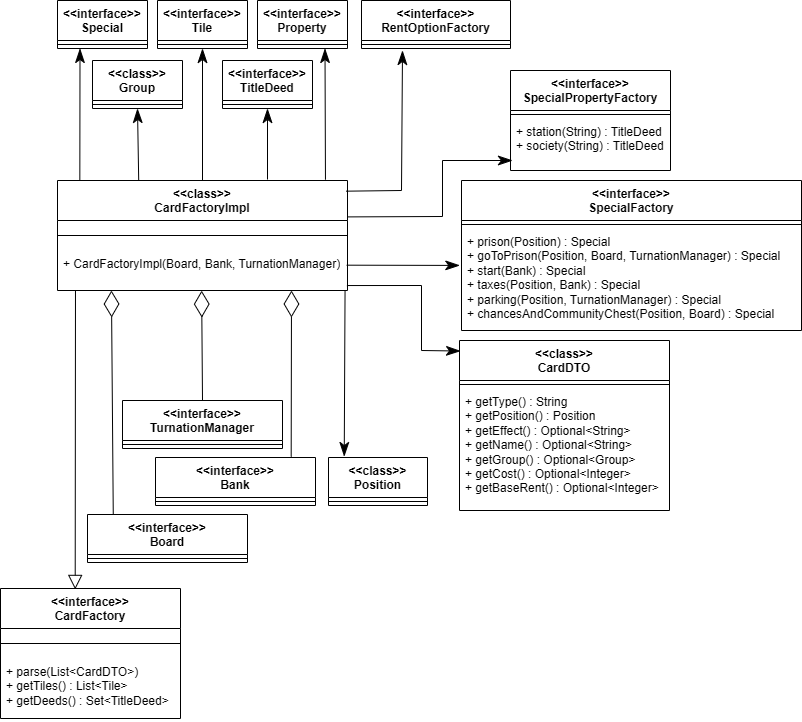
\includegraphics[width=1.3\textwidth]{img/prati/CardFactory.png}}	
    \caption{Schema UML della creazione delle tessere di gioco}
	\label{img:CardFactory}
\end{figure}

\subsubsection{File di configurazione}
\textbf{Problema}\newline
All'avvio il gioco legge dal file di configurazione (\texttt{config.yml}) le impostazioni utente (min/max giocatori, dadi, font, saldo iniziale, percorsi file, colori).\newline
Se il file è assente, malformato o contiene valori non validi, il caricamento può fallire o generare comportamenti inaspettati.\newline
Per evitare questo, è necessario validare i dati prima di creare l'istanza definitiva e, in caso di errori o incongruenze, 
ignorare la configurazione utente e ricorrere a valori di default sempre garantiti validi.
\dots\newline
\textbf{Soluzione}\newline
Per gestire in modo modulare e sicuro il caricamento delle impostazioni ho combinato due pattern:\newline
\begin{itemize}
  \item Strategy Pattern: 
        L'interfaccia \texttt{UseConfigurationFile} definisce il contratto per chi legge un file di configurazione, mentre la sua implementazione concreta si occupa di tutto il parsing YAML e della gestione delle eccezioni. \newline
        In fase di avvio, \texttt{Configuration.configureFromFile(path)} delega a questa strategia e ottiene un oggetto “grezzo” che raccoglie i valori dal file.

  \item Builder Pattern:
        A questo punto entra in gioco il builder di \texttt{Configuration}: inizializzato sui valori di default, espone metodi per applicare ciascun parametro letto da file. \newline
        Il builder è “single-use” e, quando si invoca la creazione, viene prima eseguito un controllo di validità.
        Se ci sono valori mancanti o fuori dominio, anziché propagare l'errore ritorna automaticamente alla configurazione di default.

\end{itemize}
Grazie a questo approccio, l'istanza definitiva di \texttt{Configuration} viene prodotta solo dopo aver validato ogni parametro, 
e il gioco parte sempre con un oggetto immutabile e coerente, ignorando silenziosamente eventuali configurazioni non valide.
\newline
\begin{figure}[H]
    \centering
    \makebox[1.0\textwidth]{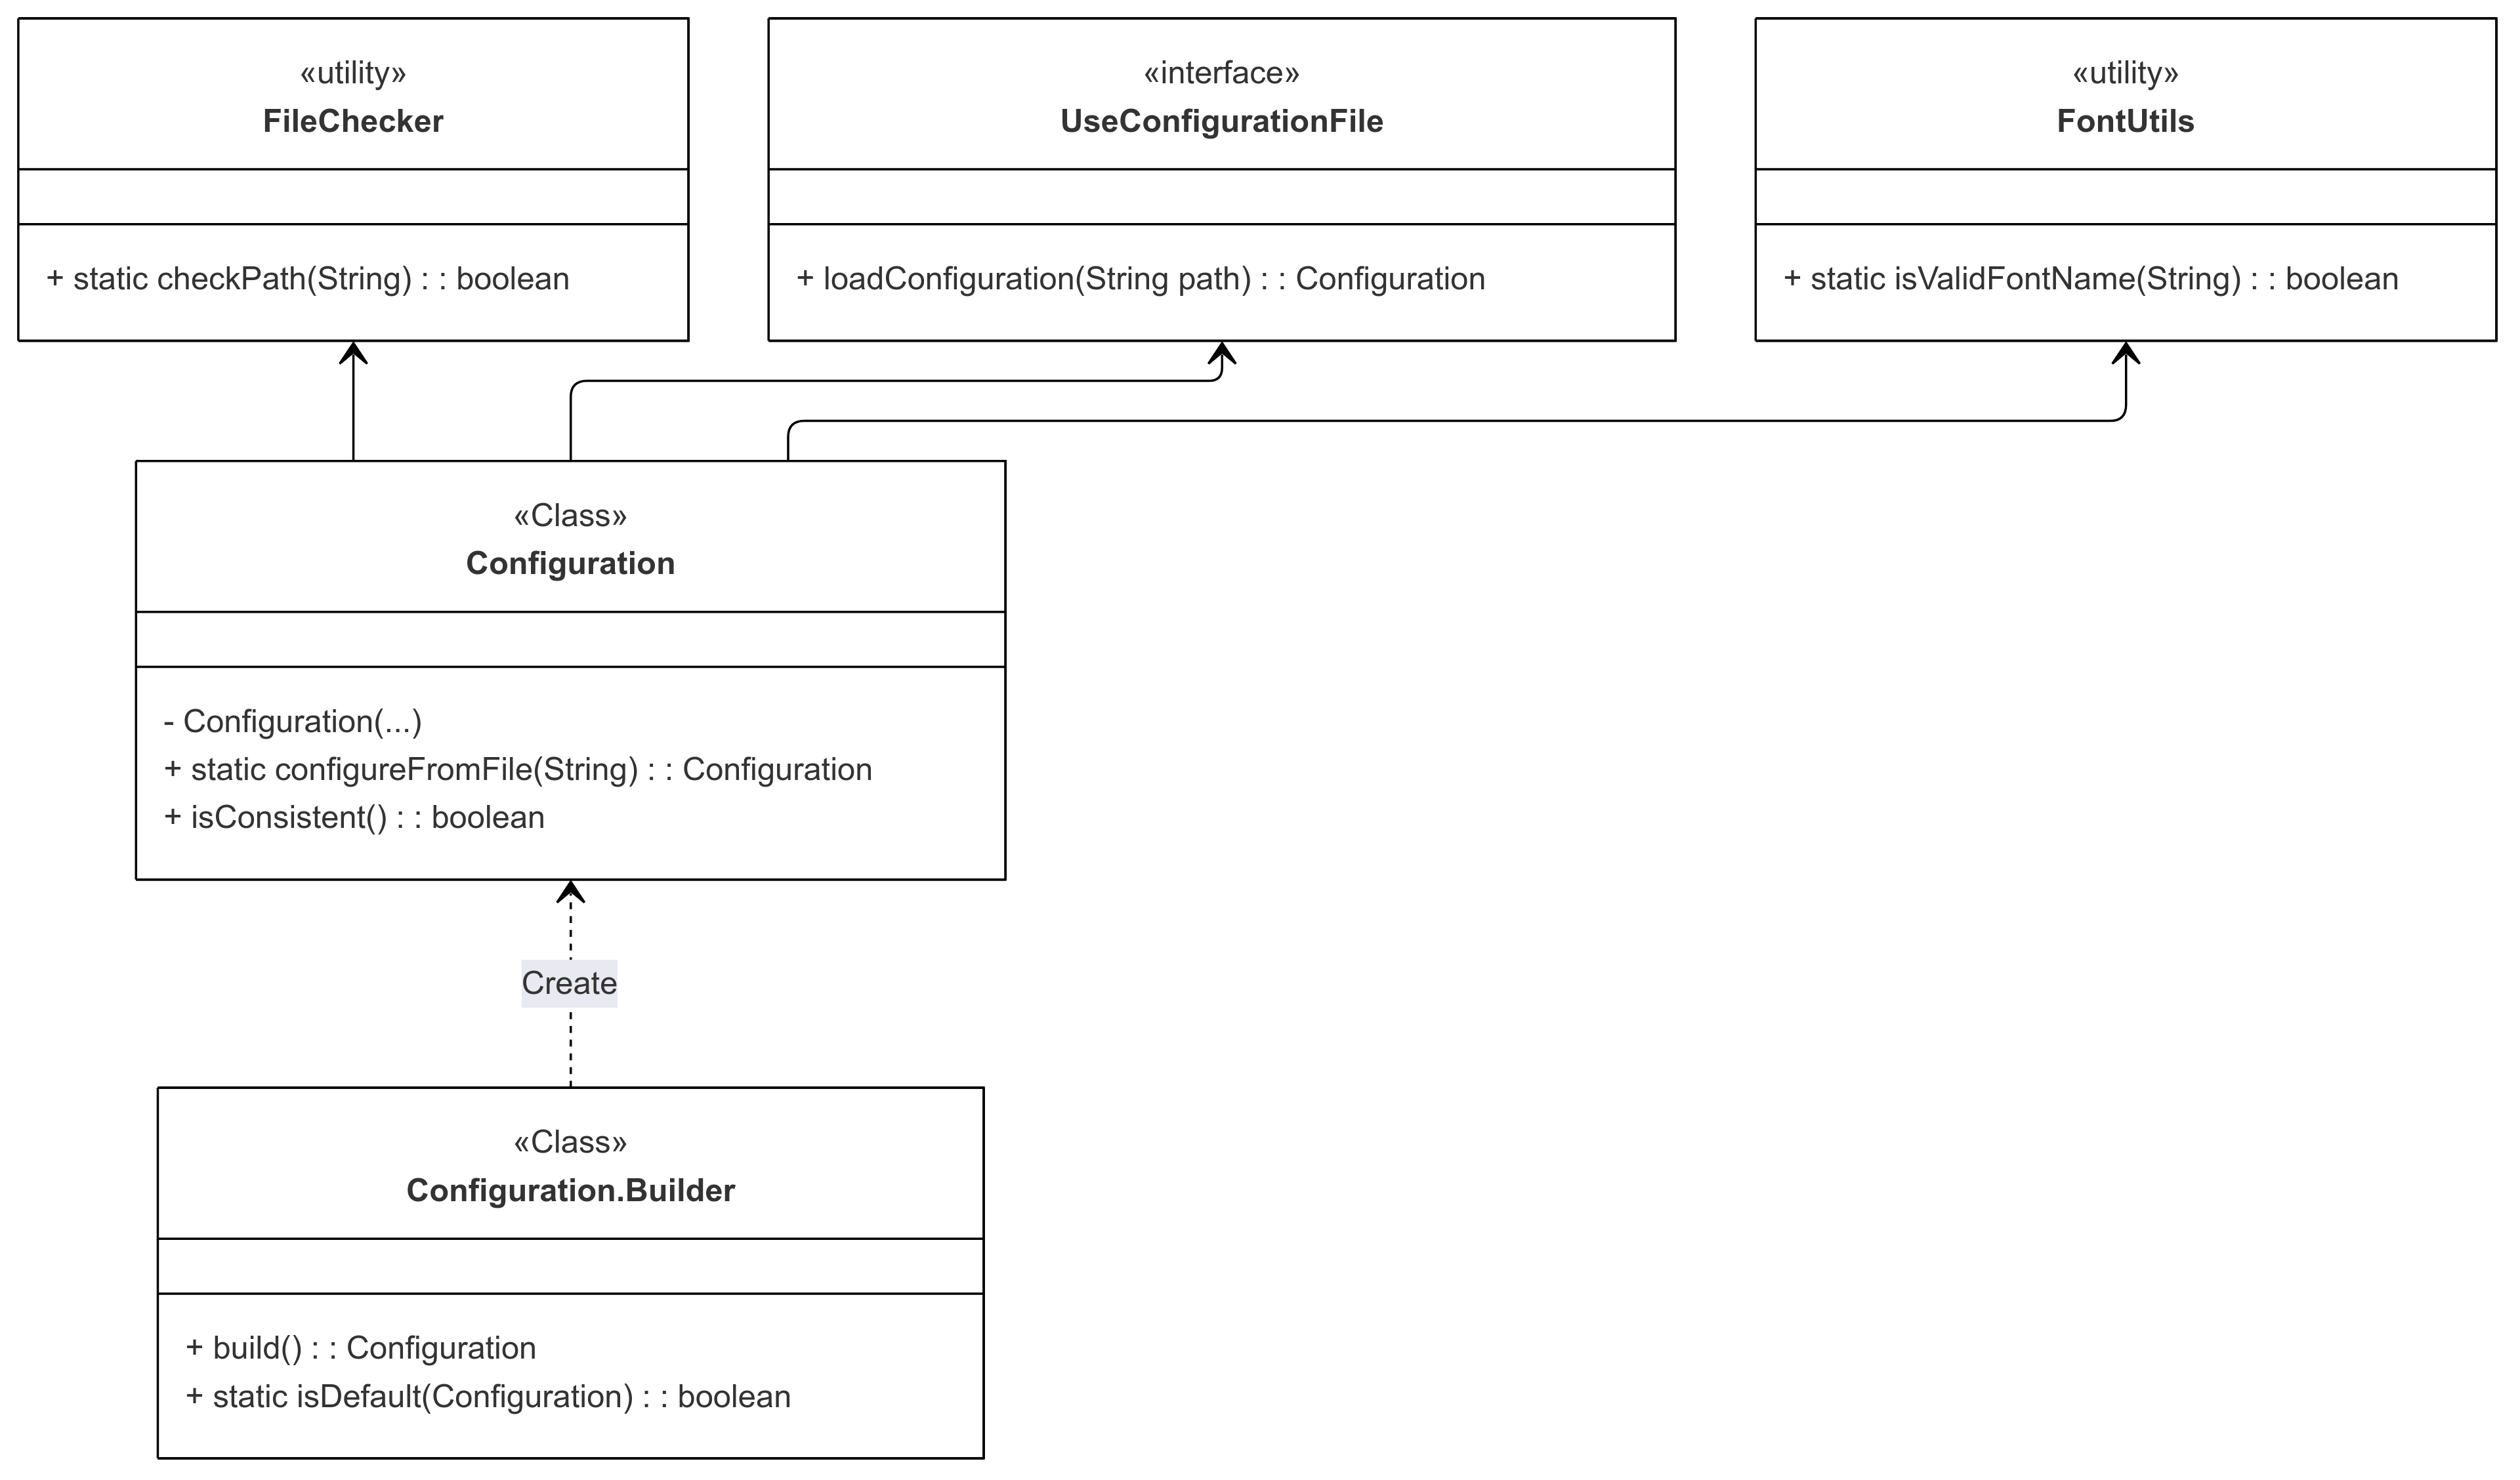
\includegraphics[width=1.3\textwidth]{img/prati/Configuration.png}}	
    \caption{Schema UML della creazione della configurazione di gioco}
	\label{img:Configuration}
\end{figure}

\subsubsection{Creazione dei conti bancari secondo la modalità di gioco}
\textbf{Problema}\newline
All'avvio della partita, per ogni giocatore occorre creare un \texttt{BankAccount} in base alla modalità di gioco selezionata (\texttt{CLASSIC} vs \texttt{INFINITY}).\newline
Serve un punto unico di creazione per evitare duplicazioni e rispettare il Principio Open/Closed (OCP).
\dots\newline
\textbf{Soluzione}\newline
Ho applicato il Factory Pattern, definendo l'interfaccia \texttt{BankAccountFactory] e una sua implementazione che, accettando al costruttore il saldo da impostare nei conti correnti 
e accettando un id e un valore di \texttt{BankAccountType} durante l'invocazione della creazione, restituisce il conto corretto.\newline
Durante il setup, il controller chiama semplicemente\newline
	\texttt{factory = new BankAccountFactoryImpl(int);}\newline
	\texttt{factory.createBankAccountByType(id, bankAccountType);}\newline
senza mai conoscere i dettagli interni.\newline
In futuro, per aggiungere nuove modalità, basterà estendere l'enum BankAccountType e aggiornare la casistica nella factory, lasciando intatto il resto dell'applicazione.\newline

\newline
\begin{figure}[H]
    \centering
    \makebox[1.0\textwidth]{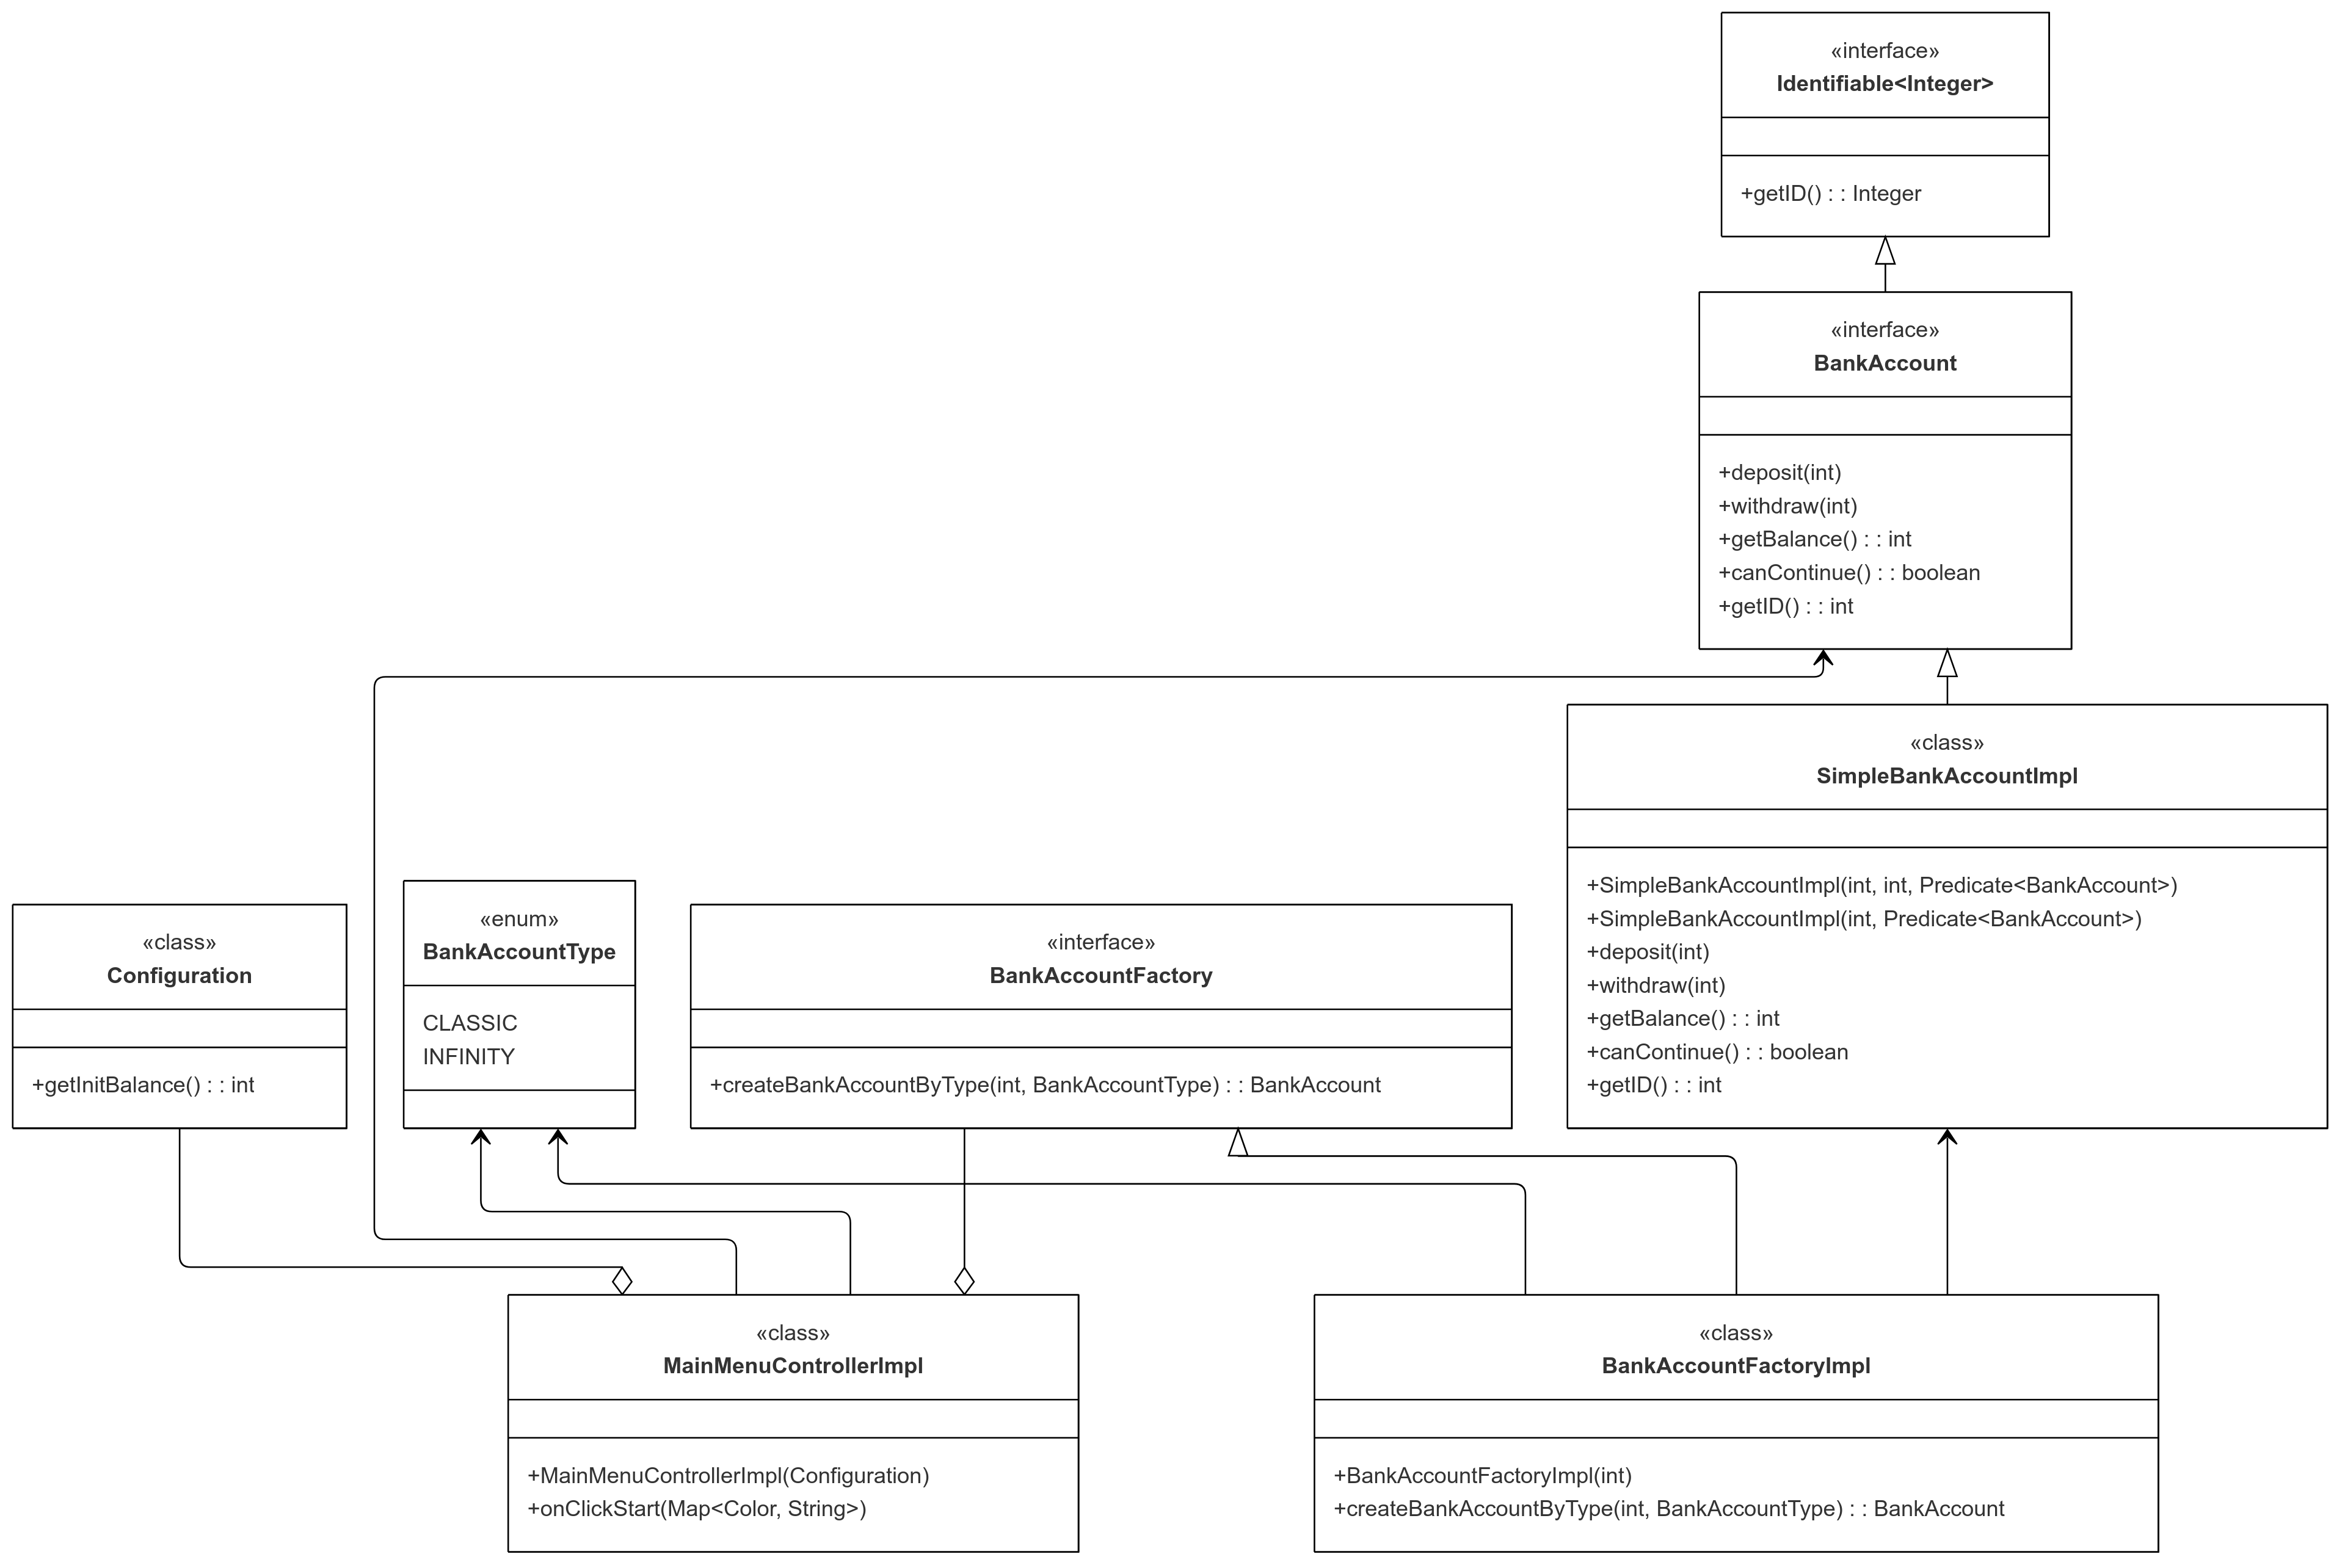
\includegraphics[width=1.3\textwidth]{img/prati/BankAccountFactory.png}}	
    \caption{Schema UML della creazione della configurazione di gioco}
	\label{img:BankAccountFactory}
\end{figure}